\chapter{Image Manipulation (2D)}

\section{Multiplanar Reconstruction}

When images are imported, InVesalius automatically shows its reconstruction
Multiplanar in the Axial, Sagittal and Coronal orientations, as well as a window for 3D manipulation.
See figure \ref{fig:mpr}.

\begin{figure}[!htb]
\centering
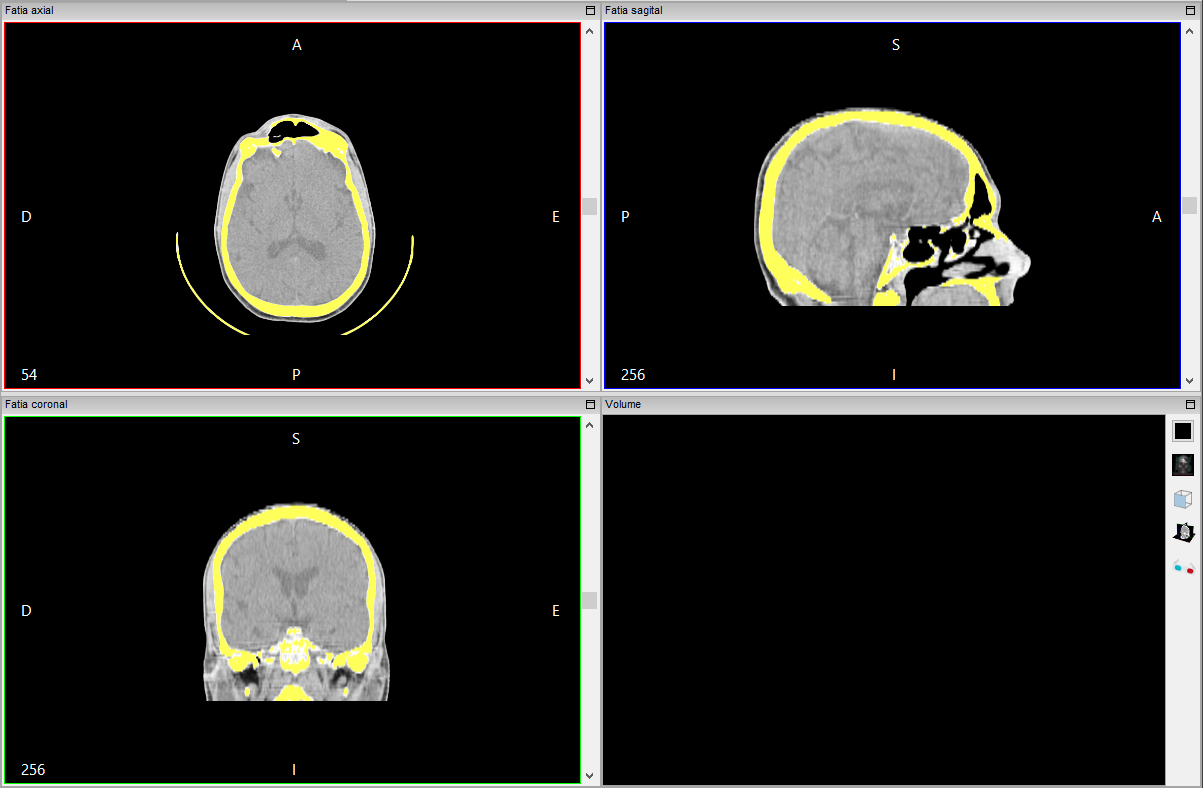
\includegraphics[scale=0.30]{multiplanar_mask_window_pt.png}
\caption{Multiplanar Reconstruction}
\label{fig:mpr}
\end{figure}

\newpage

In addition to creating a multiplanar reconstruction, InVesalius segments an image, highlighting, for example, soft tissue bones. The highlight is represented by the application of colors on a segmented structure, i.e., the colors forms a mask over an image highlighting the structure (figure \ref{fig:mpr}). This is discussed in more detail in the following chapters.


To hide the mask, use the data manager, located in the lower left corner
of the screen. Just choose the tab \textbf{Masks} and click \textbf{once} using the
\textbf{left} mouse buttom over the eye icon next to \textbf{"Mask 1"}. See figure
\ref{fig:ger_masc}.

\begin{figure}[!htb]
\centering
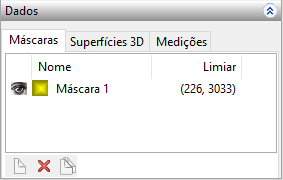
\includegraphics[scale=0.8]{data_mask_pt.png}
\caption{Mask manager}
\label{fig:ger_masc}
\end{figure}

The eye icon disappears, and the colors of the segmentation mask are hidden (figure
\ref{fig:mpr_sem_mask}).

\begin{figure}[!htb]
\centering
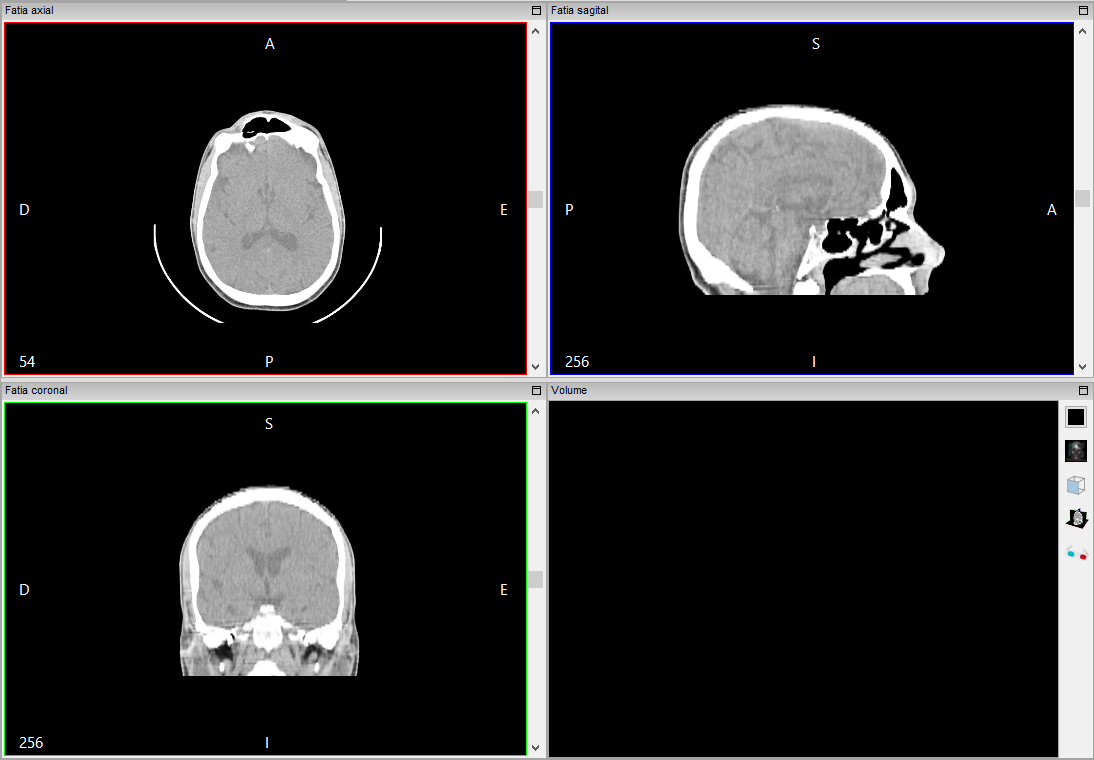
\includegraphics[scale=0.30]{multiplanar_window_pt.png}
\caption{Multiplanar reconstruction without segmentation mask}
\label{fig:mpr_sem_mask}
\end{figure}

\subsection{Axial orientation}

The axial orientation consists of cuts made transversal in relation to the region of interest, i.e. parallel cuts to the axial plane of the human body.
In figure \ref{fig:axial_corte}, an axial image of the skull region is displayed.

\begin{figure}[!htb]
\centering
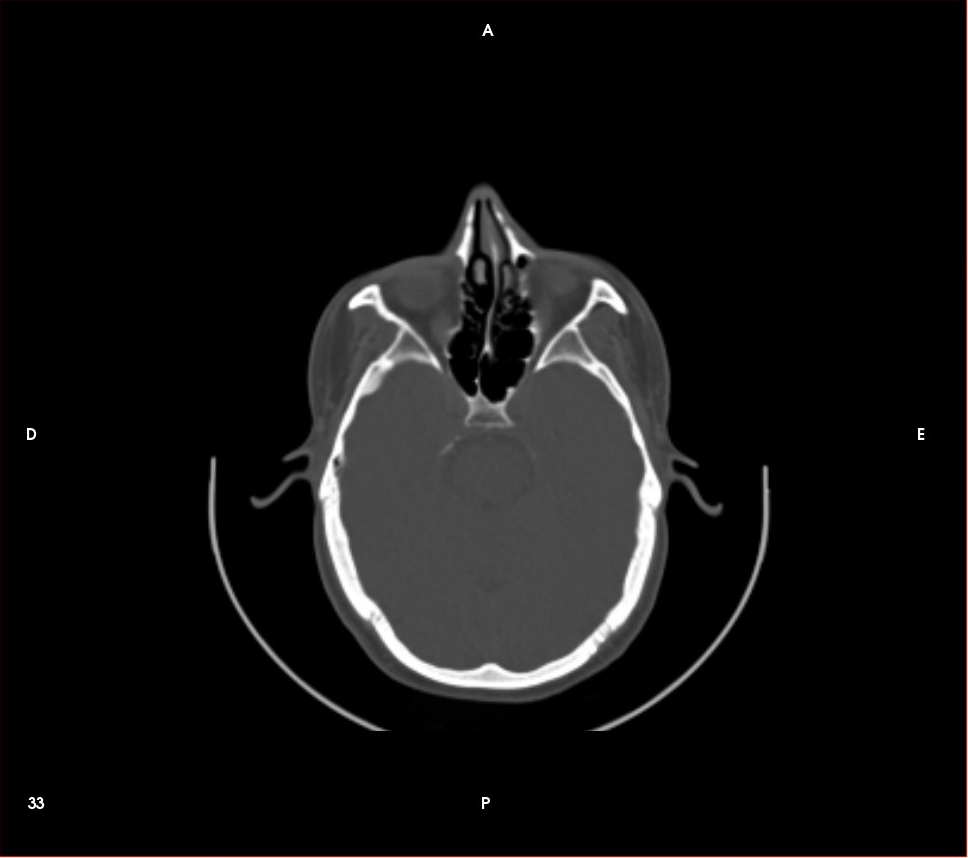
\includegraphics[scale=0.15]{axial.jpg}
\caption{Axial cut}
\label{fig:axial_corte}
\end{figure}

\subsection{Sagittal orientation}

The sagittal orientation consists of cuts made laterally in relation to the region of interest, i.e. parallel cuts to the sagittal plane of the human body, which divides it into the left and right portions.
In figure \ref{fig:sagital_slice}, a sagittal skull image is displayed.

\begin{figure}[!htb]
\centering
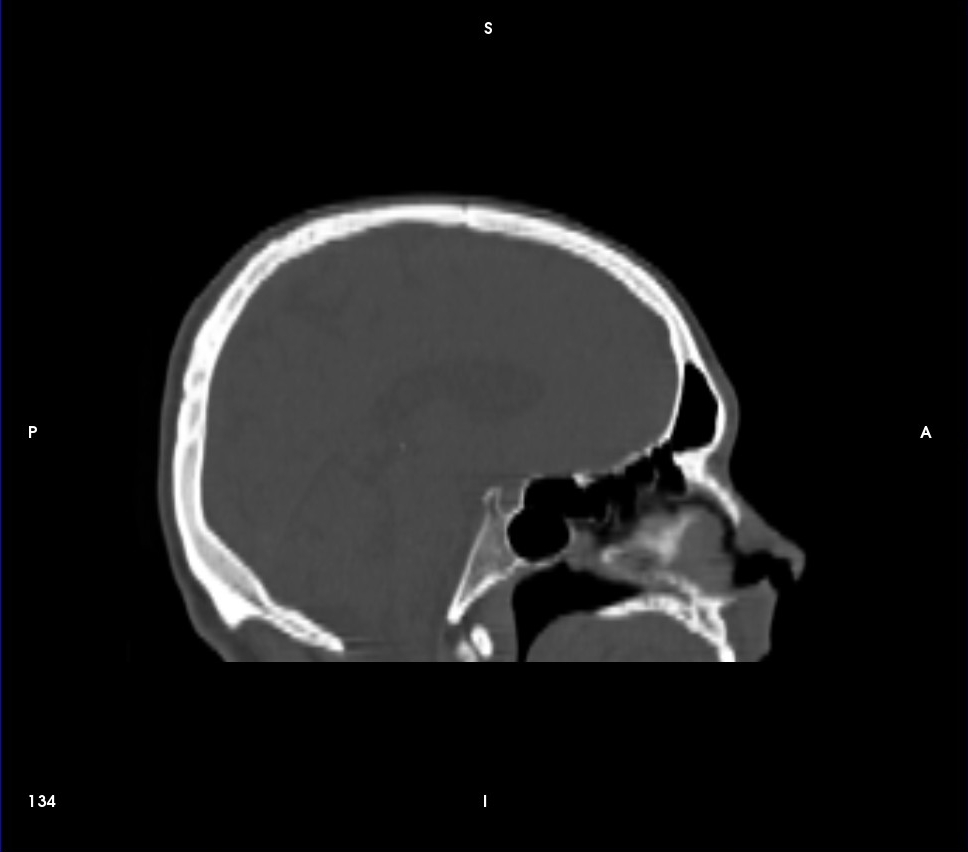
\includegraphics[scale=0.15]{sagital.jpg}
\caption{Sagittal cut}
\label{fig:sagital_slice}
\end{figure}

\newpage

\subsection{Coronal orientation}

The coronal orientation is composed of cuts parallel to the coronal plane, which divides the human body into ventral and dorsal halves.
In figure \ref{fig:coronal_slice} is displayed  a skull image in coronal orientation.

\begin{figure}[!htb]
\centering
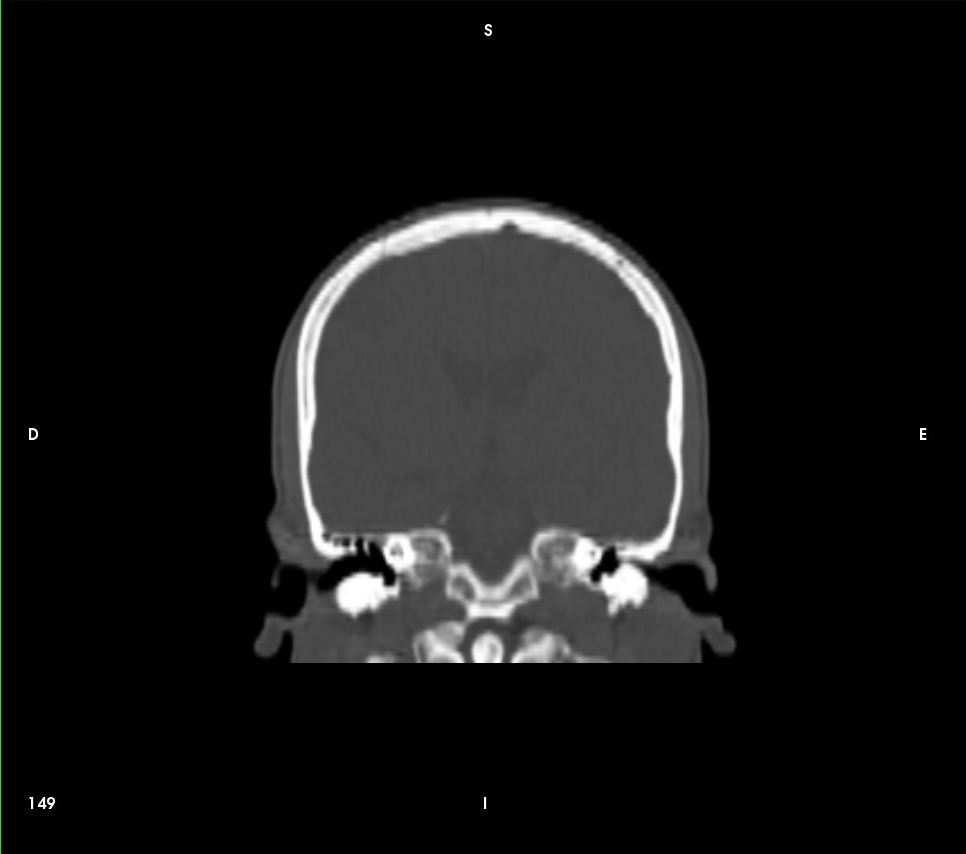
\includegraphics[scale=0.15]{coronal.jpg}
\caption{Coronal cut}
\label{fig:coronal_slice}
\end{figure}


\section{Correspondence between the axial, sagittal and coronal orientations}
\label{sec:corresp_all_orient}

To find out the common point of the images in differents orientations, simply activate the "Slices' cross intersection" feature with the shortcut icon located on the toolbar.
See figure \ref{fig:cross_icon}.

\begin{figure}[!htb]
\centering

\includegraphics[scale=1]{cross.png}
\caption{Shortcut to show common point between different orientations}
\label{fig:cross_icon}
\end{figure}

When the feature is fired, two cross segments that intersect perpendicularly are displayed on each image (figure \ref{fig:cross_all}). The intersection point of each pair of segments represents the common point between differents orientations.

\newpage

To modify the point, keep \textbf{pressed} the \textbf{left} mouse button and
\textbf{drag}. Automatically, the corresponding points will be updated in each image.

\begin{figure}[!htb]
\centering
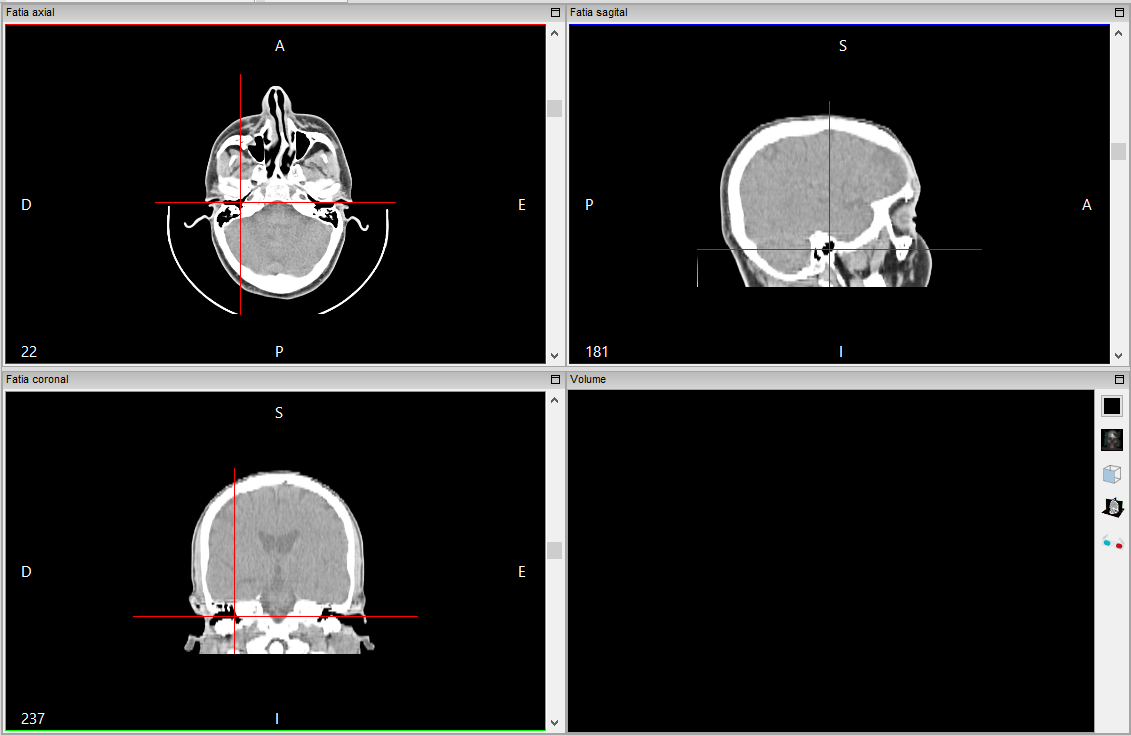
\includegraphics[scale=0.4]{multiplanar_window_cross_pt.png}
\caption{Common point between differents orientations}
\label{fig:cross_all}
\end{figure}

To disable the feature, simply click on the shortcut again (figure \ref{fig:cross_icon}). This feature can be used in conjunction with the slice editor (which will be discussed later).

\section{Interpolation}

By default the 2D images visualization are interpolated (figure~\ref{fig:interp}).a, to deactivate this feature, in menu press \textbf{View}, \textbf{Interpolated slices} (figure~\ref{fig:menu_interpoleted_image_pt}). In this way it will be possible to visualize each pixel individually as shown in the figure~\ref{fig:interp}.b.

\textbf{Note: This interpolation is for visualization purposes only, not directly influencing segmentation or 3D surface generation.}

\begin{figure}[!htb]
\centering
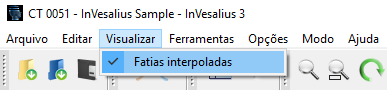
\includegraphics[scale=0.7]{menu_interpoleted_image_pt.png}
\caption{Menu to disable and enable interpolation}
\label{fig:menu_interpoleted_image_pt}
\end{figure}


\begin{figure}[!htb]
  \centering
  \subfloat[Interpolated]{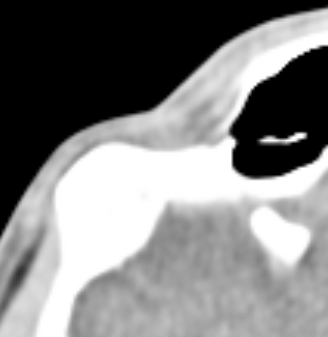
\includegraphics[width=0.4\textwidth]{axial_interpoleted.png}}  \qquad
  \subfloat[Non-interpolated]{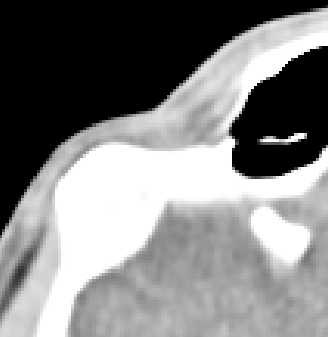
\includegraphics[width=0.4\textwidth]{axial_not_interpoleted.png}}
  \hfill
  \caption{Interpolated and non-interpolated image visualization.}
  \label{fig:interp}
\end{figure}

\section{Move}

To move an image on the screen, the toolbar's "Move" shortcut icon can be used (figure
\ref{fig:move_icon}). Click on the icon to activate the feature and then with the \textbf{left} mouse button on the image, \textbf{drag} it to the desired direction. The figure \ref{fig:move_img} shows a displaced (moved) image.

\begin{figure}[!htb]
\centering

\includegraphics[scale=0.25]{tool_translate_original.png}
\caption{Shortcut to move images}
\label{fig:move_icon}
\end{figure}

\begin{figure}[!htb]
\centering
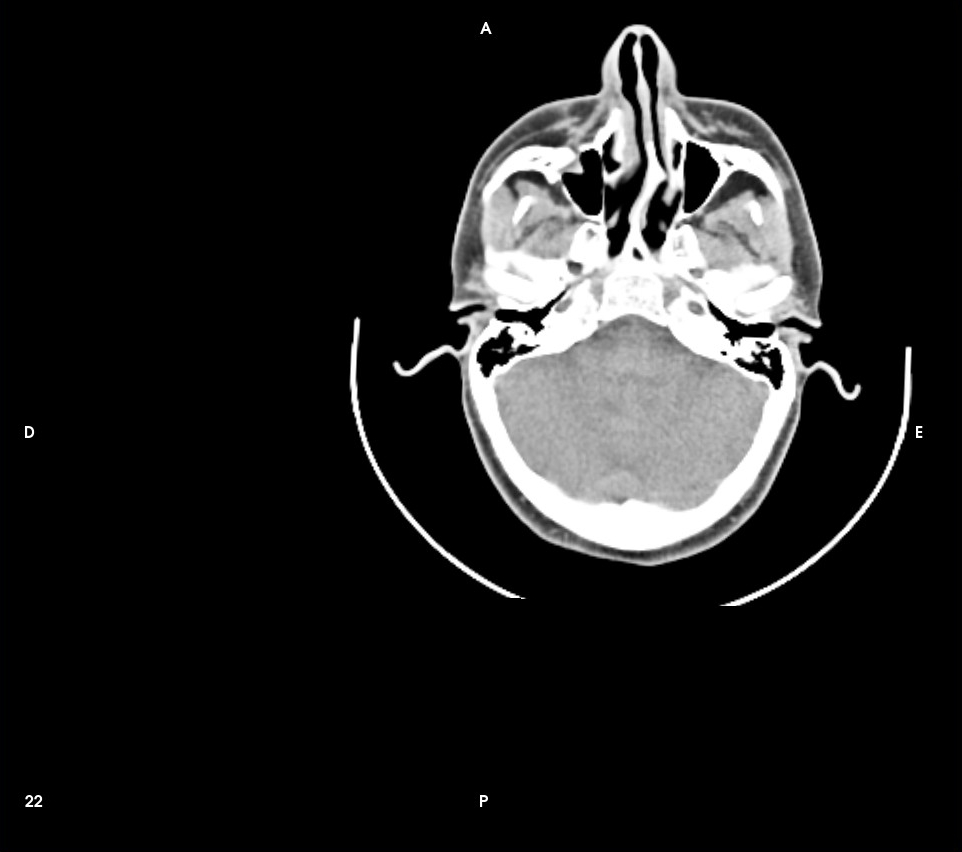
\includegraphics[scale=0.25]{axial_pan.jpg}
\caption{Displaced image}
\label{fig:move_img}
\end{figure}

\section{Rotate}

The image rotation can be activated by the toolbar's "Rotate" shortcut icon (figure \ref{fig:rot_icon}). To rotate an image, click on the icon and then with the \textbf{left} mouse button press on the image, \textbf{drag} clockwise or anticlockwise, depending on the desired direction of rotation.

\begin{figure}[!htb]
\centering

\includegraphics[scale=0.25]{tool_rotate_original.png}
\caption{Shortcut to rotate images}
\label{fig:rot_icon}
\end{figure}

\begin{figure}[!htb]
\centering
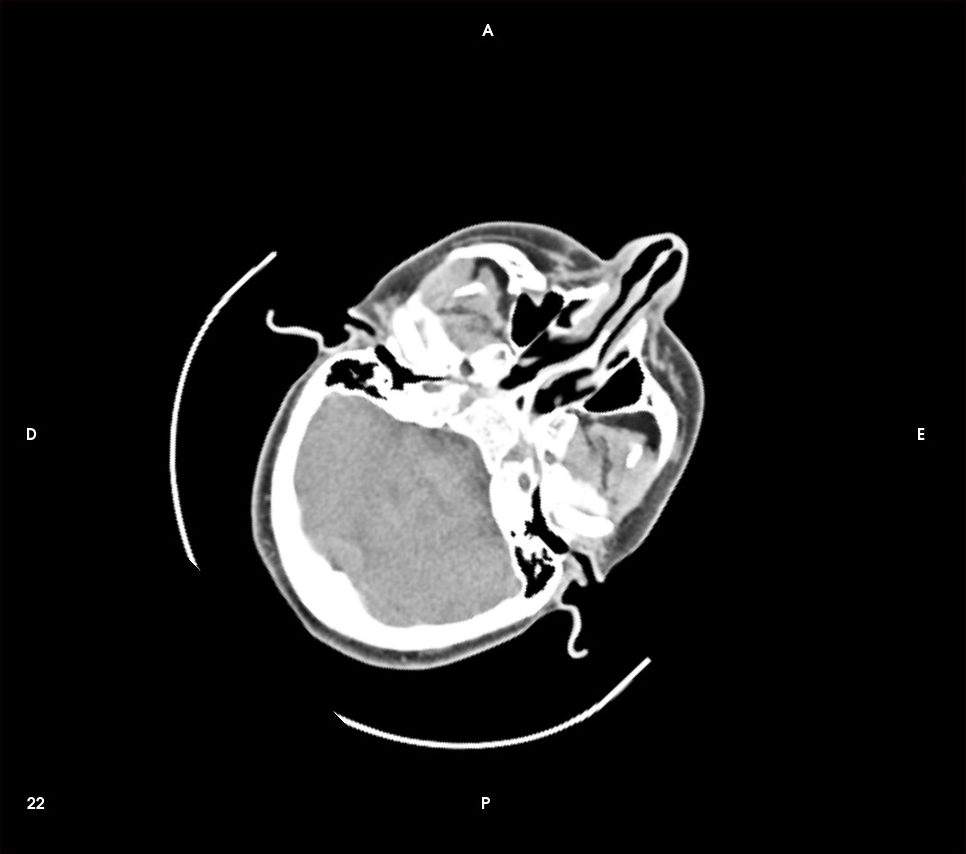
\includegraphics[scale=0.25]{axial_rotate.jpg}
\caption{Rotated image}
\label{fig:rotate_all}
\end{figure}

\section{Zoom}

In InVesalius, there are different ways to enlarge an image. You can maximize the desired orientation window, apply zoom directly to the image, or select the region of the image to enlarge.

\subsection{Maximizing orientation windows}

As we already know, the main InVesalius window is divided into 4 subwindows: axial, sagittal, coronal and 3D. Each of these can be maximized to occupy the entire area of the main window. To do this, simply \textbf{left} mouse click on the subwindow icon located in the \textbf{upper right corner} (figure \ref{fig:maximize_window}). To restore a maximized window to its previous size, simply click the icon again.

\begin{figure}[!htb]
\centering
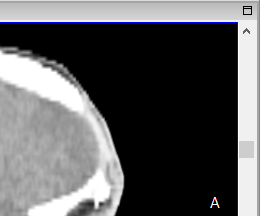
\includegraphics[scale=0.6]{maximize_sagital_mpr.png}
\caption{Detail of a sub-window (Note the maximize icon in the upper right corner)}
\label{fig:maximize_window}
\end{figure}

\subsection{Enlarging or reducing an image}

To enlarging or reducing an image, click on the zoom shortcut icon in the toolbar (figure \ref{fig:zoom_icon}). Hold down the \textbf{left} mouse button on the image and \textbf{drag} the mouse to \textbf{top} if you want to enlarge it, or \textbf{down}, if you want to reduce it.

\begin{figure}[!htb]
\centering

\includegraphics[scale=0.25]{tool_zoom_original.png}
\caption{Zoom shortcut}
\label{fig:zoom_icon}
\end{figure}

%\begin{figure}[!htb]
%\centering
%\includegraphics[scale=0.2]{ScreenHunter_76Dec311201_.jpg}
%\caption{Imagem com \textit{Zoom} aplicado}
%\label{fig:zoom_}
%\end{figure}

\subsection{Enlarging an Image Area}

To enlarging a certain image area, click on the "Zoom based on selection" icon in the toolbar (figure \ref{fig:zoom_icon_loc}). Position the mouse pointer at the start position of the selection, click and hold the \textbf{left} mouse button and \textbf{drag} it to the end selection position, forming a rectangle (figure \ref{fig:zoom_select}). Once the left mouse button is released, the zoom operation will be applied to the selected region (figure \ref{fig:zoom_applied}).

\begin{figure}[!htb]
\centering

\includegraphics[scale=0.25]{tool_zoom_select_original.png}
\caption{Zoom based on selection shortcut}
\label{fig:zoom_icon_loc}
\end{figure}

\begin{figure}[!htb]
\centering
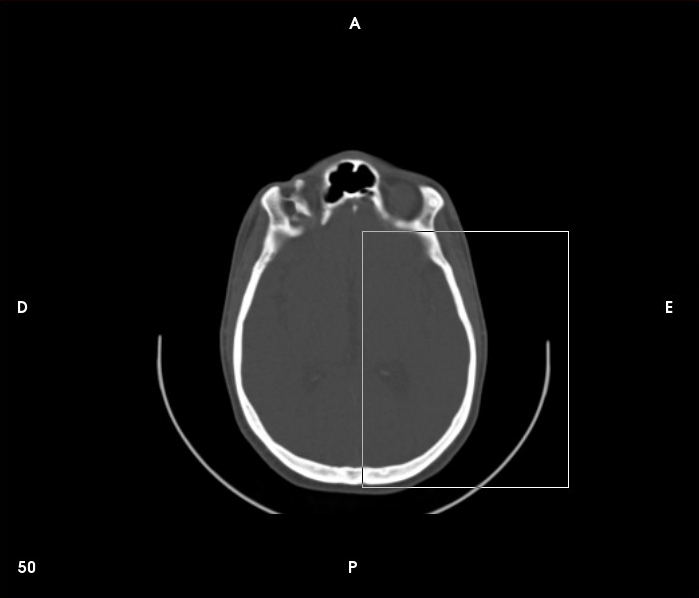
\includegraphics[scale=0.25]{tool_zoom_select_image.jpg}
\caption{Area selected for zoom}
\label{fig:zoom_select}
\end{figure}

\begin{figure}[!htb]
\centering
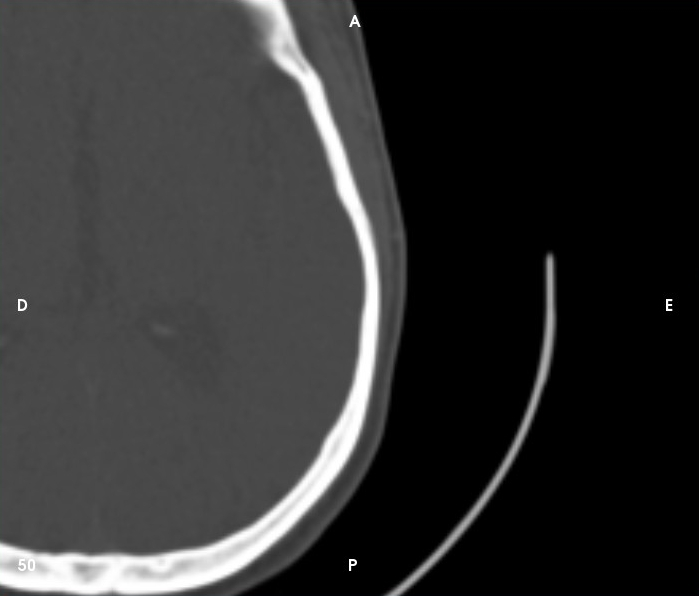
\includegraphics[scale=0.25]{tool_image_with_zoom.jpg}
\caption{Enlarged Image}
\label{fig:zoom_applied}
\end{figure}


\section{Brightness and contrast (Windows)}
\label{sec:ww_wl}

To improve images visualization, the feature \textit{window width} and \textit{window level} can be used, popularly known as "brightness and contrast" or "window" (for radiologists). With this feature, it is possible to set the range of the gray scale (\textit{window level}) and the width of the scale (\textit{window width}) to be used to display the images.

The feature can be triggered by the "Contrast" shortcut icon in the toolbar. See figure \ref{fig:window_level_shortcut}.

\begin{figure}[!htb]
\centering

\includegraphics[scale=0.70]{tool_contrast_original.png}
\caption{Brightness and contrast shortcut}
\label{fig:window_level_shortcut}
\end{figure}

To increase the brightness, hold down the \textbf{left} mouse button and \textbf{drag} horizontally to the right. To decrease the brightness, simply drag the mouse to the left. The contrast can be changed by dragging the mouse (with the \textbf{left} button pressed) vertically: up to increase, or down to decrease the contrast.

To disable the feature, click again on the shortcut icon (figure \ref{fig:window_level_shortcut}).

You can use preset brightness and contrast patterns. The table \ref{tab:window_level} lists some tissues types with their respective brightness and contrast values for the image. To use the presets patterns, position the mouse cursor over the image and \textbf{right-click} to open a context menu on it. When the menu opens, select \textbf{Window width and level}, and then click on the preset option, according to the tissue type, as shown in the figure \ref{fig:window_level}.

\begin{figure}[!htb]
\centering
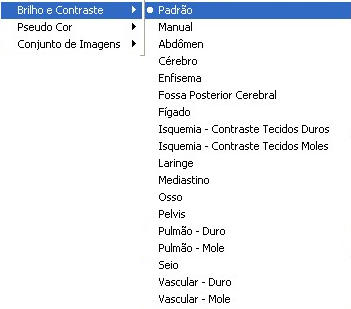
\includegraphics[scale=0.40]{menu_window_and_level_pt.png}
\caption{Context menu for brightness and contrast selection}
\label{fig:window_level}
\end{figure}

\begin{table}[h]
\centering
\caption{Brightness and contrast values for some tissues}
\begin{tabular}{lcc}\\
\hline % este comando coloca uma linha na tabela
Tissue & Brightness & Contrast\\
\hline
\hline
Default & Exam & Exam\\
Manual & Changed & Changed\\
Abdomen & 350 & 50\\
Bone & 2000 & 300\\
Brain & 80 & 40\\
Brain posterior fossa & 120 & 40\\
Contour & 255 & 127\\
Emphysema & 500 & -850\\
Ischemia - Hard, non contrast & 15 & 32\\
Ischemia - Soft, non contrast & 80 & 20\\
Larynx & 180 & 80\\
Liver & 2000 & -500\\
Lung Hard & 1000 & -600\\
Lung Soft & 1600 & -600\\
Mediastinum & 350 & 25\\
Pelvis & 450 & 50\\
Sinus & 4000 & 400\\
Vasculature - Hard & 240 & 80\\
Vasculature - Soft & 680 & 160\\
\hline
\end{tabular}
\label{tab:window_level}
\end{table} 

\begin{figure}
  \centering
  \subfloat[Bone]{\label{fig:contrast_bone}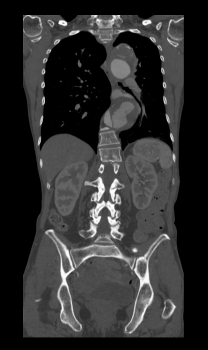
\includegraphics[width=0.4\textwidth]{contraste_osso}}
  \subfloat[Lung]{\label{fig:contrast_isq}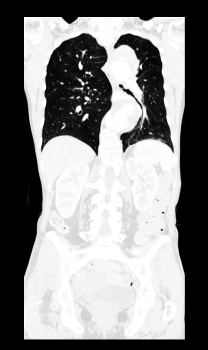
\includegraphics[width=0.4\textwidth]{contraste_pulmao}}
  \caption{Different types of brightness and contrast}
  \label{fig:two_window_level}
\end{figure}


\section{Pseudo color}

Another feature to improve the visualization of the images is the pseudo color. They replace gray levels by color, or by inverted gray levels. In the latter case, previously clear regions of the image become darker and vice versa.

To change the view using a pseudo color, position the mouse cursor over the image and \textbf{right-click} to open a context menu on it. When the menu opens, select the entry \textbf{Pseudo color}, and then click on the desired pseudo color option, as shown in the figure \ref{fig:pseudo_color}.

\begin{figure}[H]
\centering
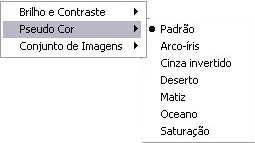
\includegraphics[scale=0.40]{pseudo_menu_pt.png}
\caption{Pseudo Color}
\label{fig:pseudo_color}
\end{figure}

Figures \ref{fig:image_default} through \ref{fig:image_saturation} exemplify the various pseudo color options available.\\

\begin{figure}[H]
\centering
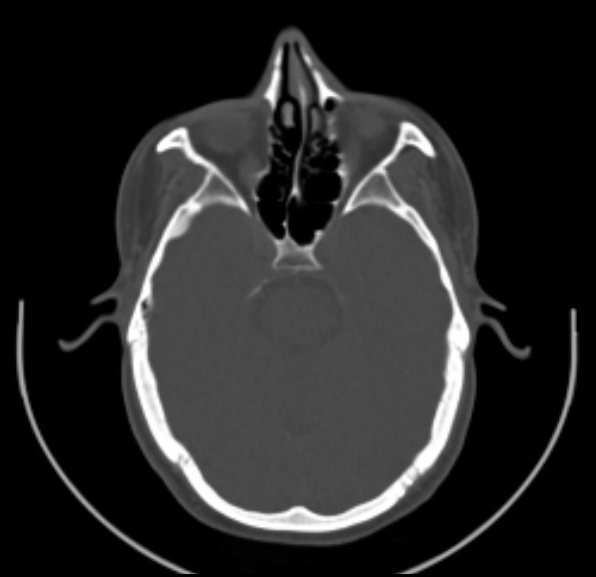
\includegraphics[scale=0.30]{pseudo_default.jpg}
\caption{Default}
\label{fig:image_default}
\end{figure}

\begin{figure}[H]
\centering
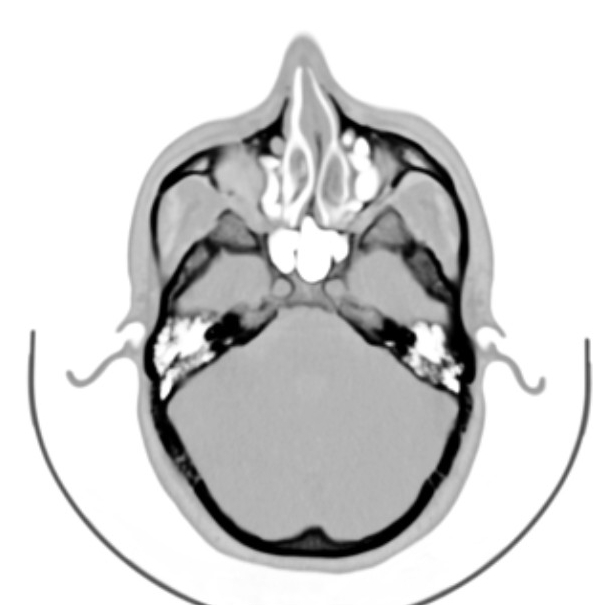
\includegraphics[scale=0.30]{pseudo_inverse.jpg}
\caption{Inverted Gray Image}
\label{fig:image_inverted}
\end{figure}

\begin{figure}[H]
\centering
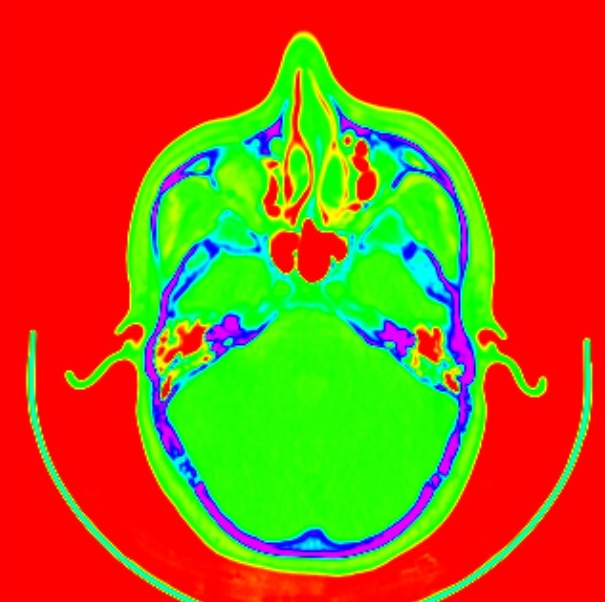
\includegraphics[scale=0.30]{pseudo_rainbow.jpg}
\caption{Rainbow}
\label{fig:image_arc}
\end{figure}

\begin{figure}[H]
\centering
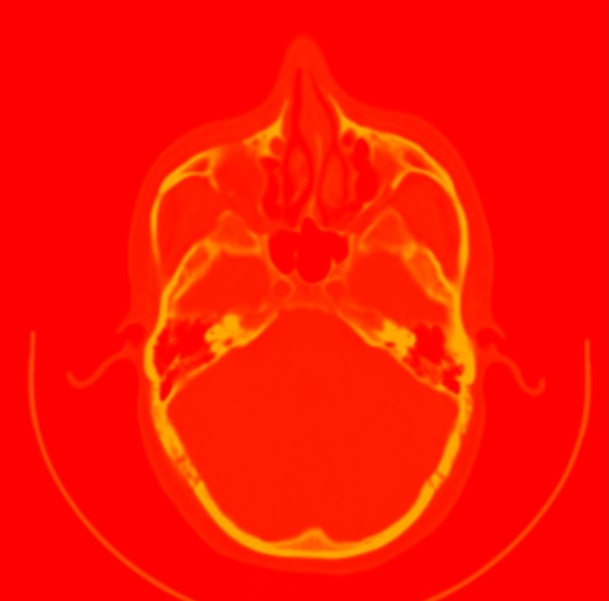
\includegraphics[scale=0.30]{pseudo_desert.jpg}
\caption{Desert}
\label{fig:image_desert}
\end{figure}

\begin{figure}[H]
\centering
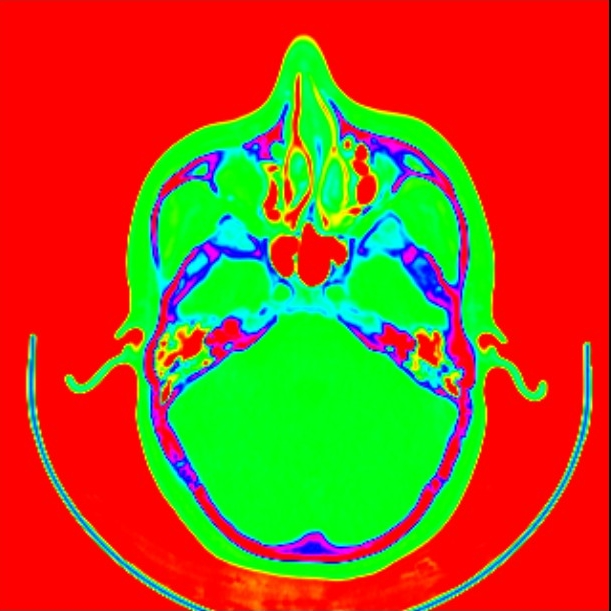
\includegraphics[scale=0.30]{pseudo_hue.jpg}
\caption{Hue}
\label{fig:image_matiz}
\end{figure}

\begin{figure}[H]
\centering
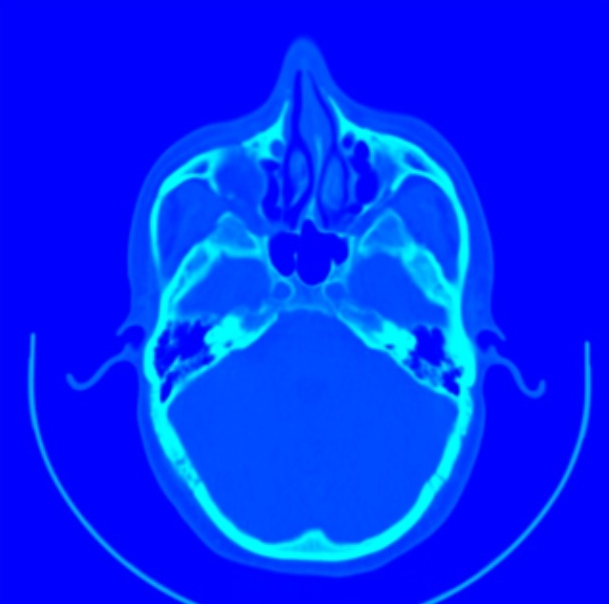
\includegraphics[scale=0.30]{pseudo_ocean.jpg}
\caption{Ocean}
\label{fig:image_ocean}
\end{figure}

\begin{figure}[H]
\centering
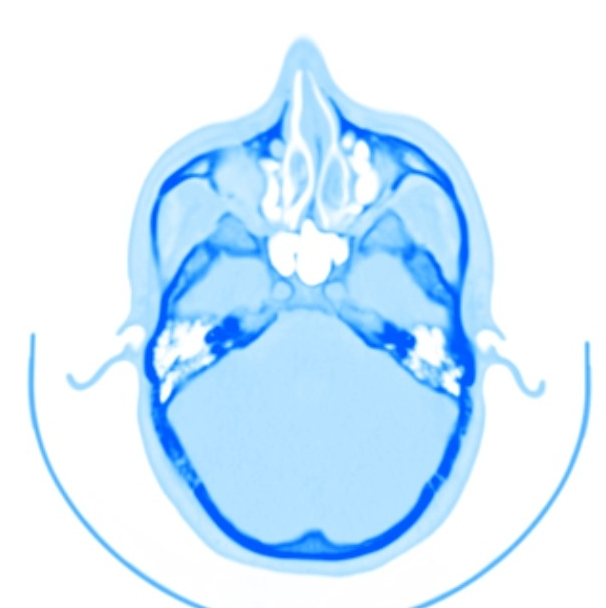
\includegraphics[scale=0.30]{pseudo_saturation.jpg}
\caption{Saturation}
\label{fig:image_saturation}
\end{figure}

\newpage

\section{Projection type}

It is possible to change the projection type of the 2D images, in addition to the normal mode, InVesalius has six types of projections that can be accessed as follows: Place the mouse over the image and \textbf{rigth-click} to open a context menu on it. When the menu opens, select the projection type option, and then click on the desired projection option, as shown in the figure ~\ref{fig:menu_proj}.

\begin{figure}[H]
\centering
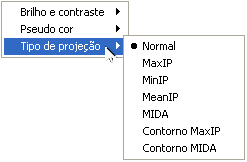
\includegraphics[scale=0.60]{menu_projection_pt.png}
\caption{Projection Type menu}
\label{fig:menu_proj}
\end{figure}

\subsection{Normal}

Normal mode is the default view, i.e. without any type of projection, originally when the image was acquired or customized previously with either brightness and contrast or pseudo color. As shown in figure ~\ref{fig:proj_normal}.

\begin{figure}[H]
\centering
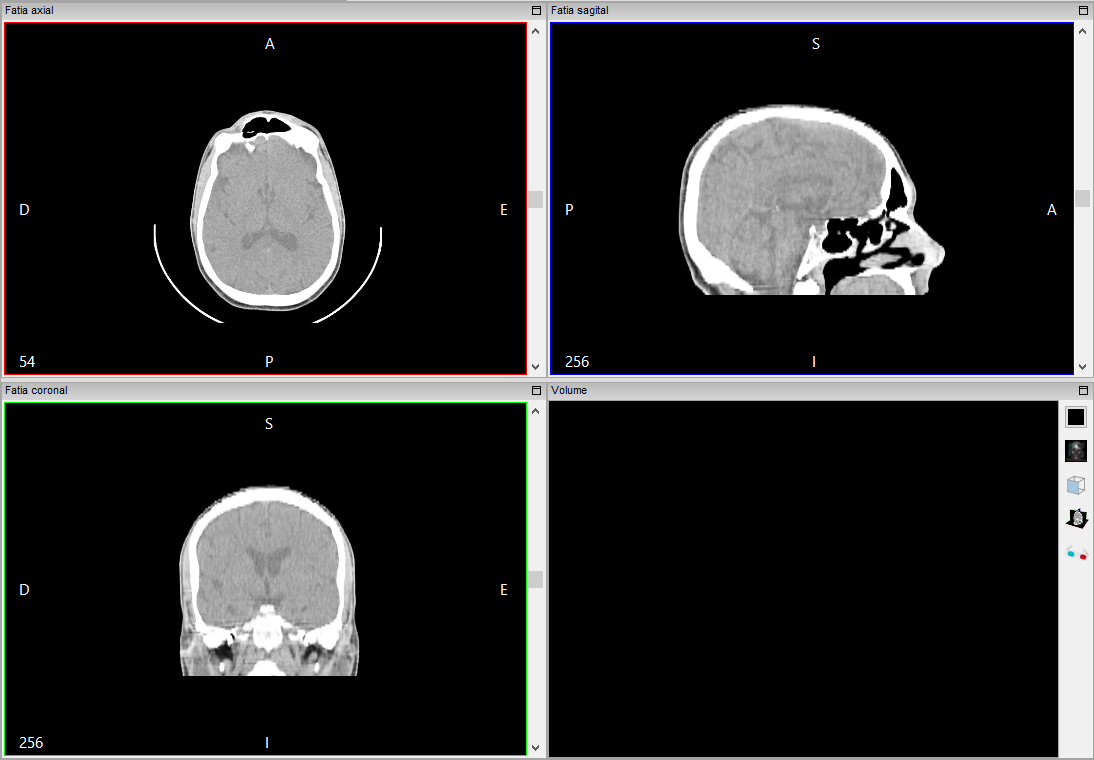
\includegraphics[scale=0.40]{multiplanar_window_pt.png}
\caption{Normal projection}
\label{fig:proj_normal}
\end{figure}

\subsection{MaxIP}
\label{sec:max_ip}
MaxIP is also known as MIP (\textit{Maximum Intensity Projection}), the method selects only voxels that have maximum intensity among the visited ones as shown in figure ~\ref{fig:proj_maxip}. According to the amount or "depth" of MaxIP each voxel is visited in order of overlap, for example, to select MaxIP of the pixel $(0,0)$ consisting of 3 slices it is necessary to visit the pixel $(0,0)$ of slices $(1,2,3)$ and select the highest value.

\begin{figure}[H]
\centering
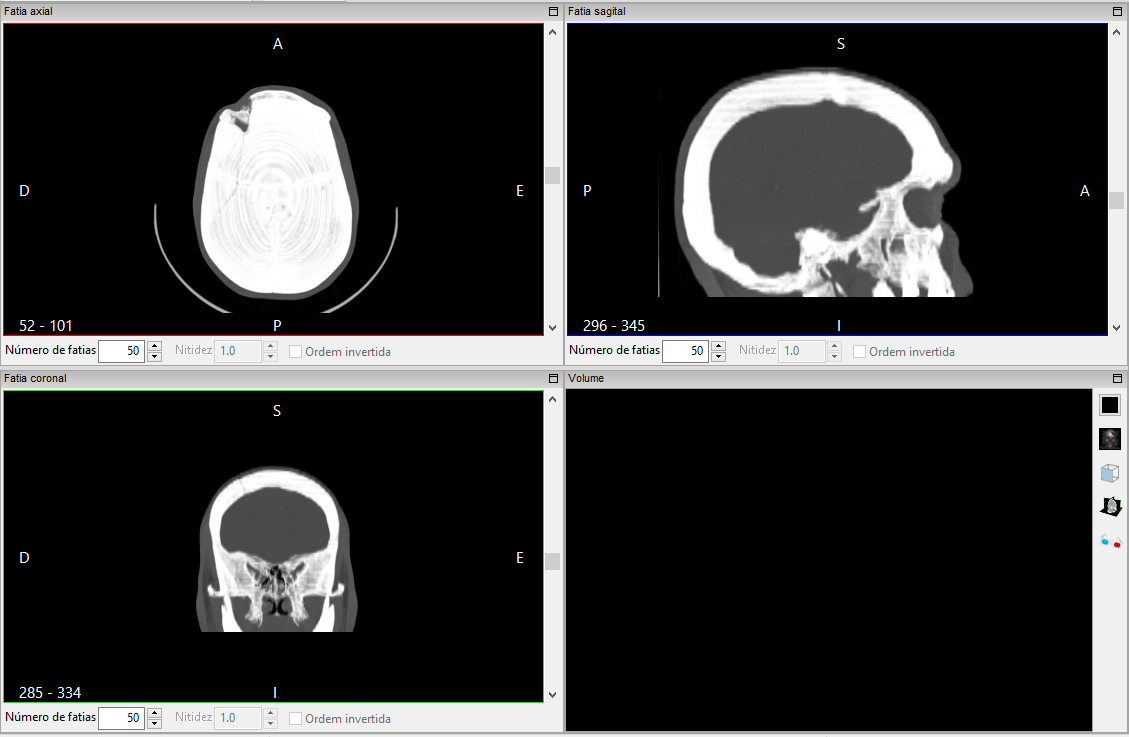
\includegraphics[scale=0.40]{multiplanar_window_maxip_pt.png}
\caption{MaxIP or MIP projection}
\label{fig:proj_maxip}
\end{figure}

As shown in the figure~\ref{fig:proj_maxip_qtd}, the number of images that will be composed of MaxIP is set at the bottom of each orientation image.

\begin{figure}[H]
\centering
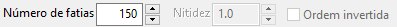
\includegraphics[scale=0.80]{multiplanar_window_maxip_number_pt.png}
\caption{Selection the amount of images that composes the MaxIP or MIP}
\label{fig:proj_maxip_qtd}
\end{figure}

\subsection{MinIP}

Unlike MaxIP, MinIP (\textit{Minimun Intensity Projection}) selects only the voxels that have minimal internsity among the visited ones, an example is shown in figure~\ref{fig:proj_minIP}. The image number selection that will compose the projection is made at the bottom of each orientation image as shown in figure~\ref{fig:proj_maxip_qtd}.

\begin{figure}[H]
\centering
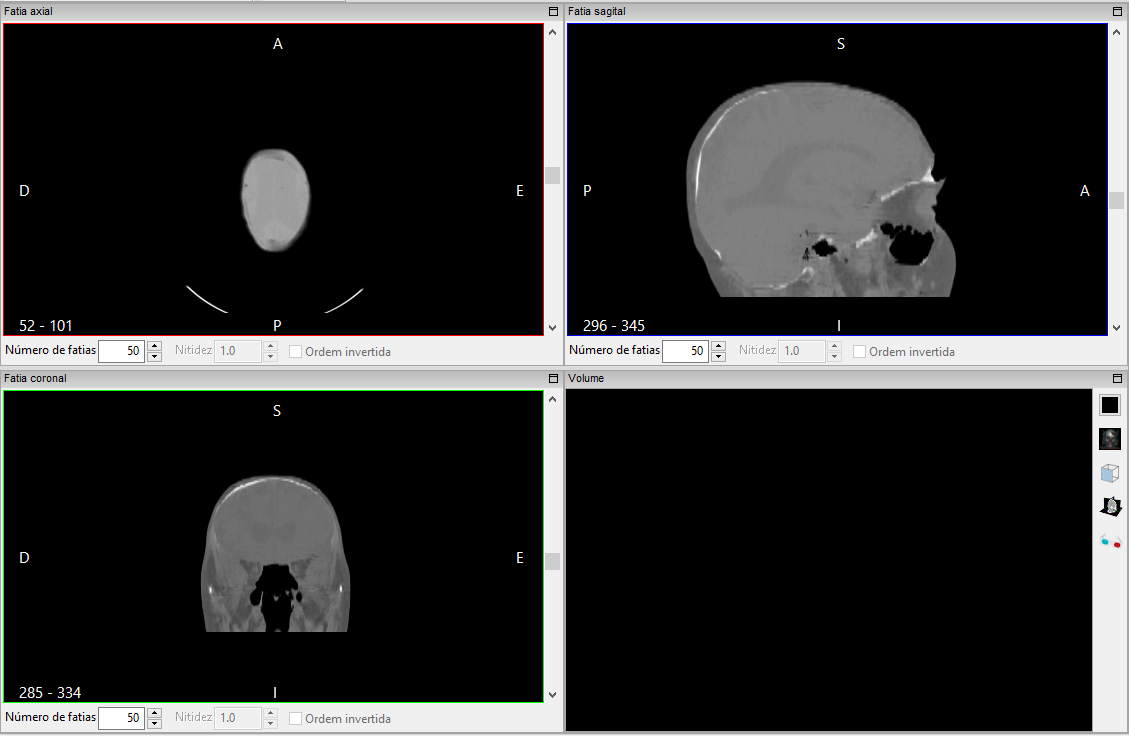
\includegraphics[scale=0.40]{multiplanar_window_minip_pt.png}
\caption{MinIP projection}
\label{fig:proj_minIP}
\end{figure}

\subsection{MeanIP}
The MeanIP (\textit{Mean Intensity Projection}) technique which is shown in the figure~\ref{fig:proj_meanIP} composes the projection by averaging the voxels visited. The voxels are visited in the same way as the MaxIP and MinIP methods. It is also possible to define how many images will compose the projection at the bottom of the image of each orientation as shown in the figure~\ref{fig:proj_maxip_qtd}.

\begin{figure}[H]
\centering
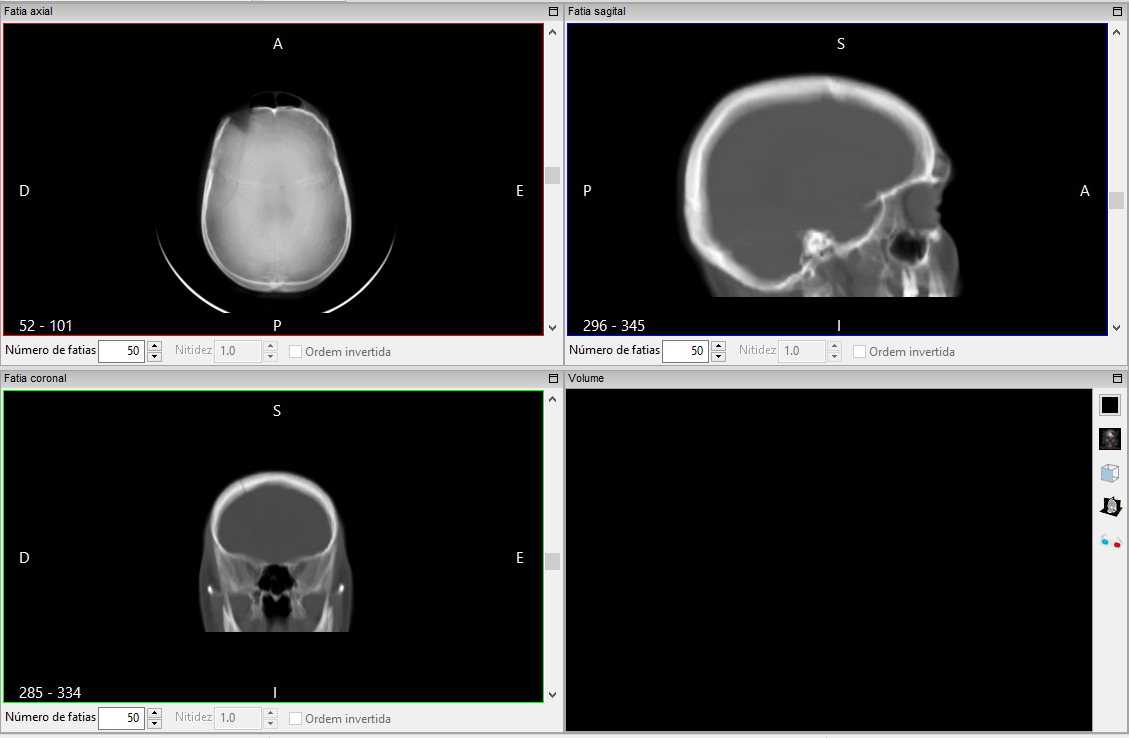
\includegraphics[scale=0.40]{multiplanar_window_mean_pt.png}
\caption{MeanIP projection}
\label{fig:proj_meanIP}
\end{figure}

\subsection{MIDA}
\label{sub:mida}
The MIDA (\textit{Maximum Intensity Difference Accumulation}) technique projects an image taking into account only voxels that have local maximum values. From each pixel a ray is simulated towards the volume, each voxel is intercepted by each of these rays reaching the end of the volume, each of these voxels visited has its accumulated value, but are taken into account only if the value is greater than previously visited values. Like MaxIP, you can select how many images are used to accumulate the values. The figure ~\ref{fig:proj_MIDA} shows an example of MIDA projection.

\begin{figure}[H]
\centering
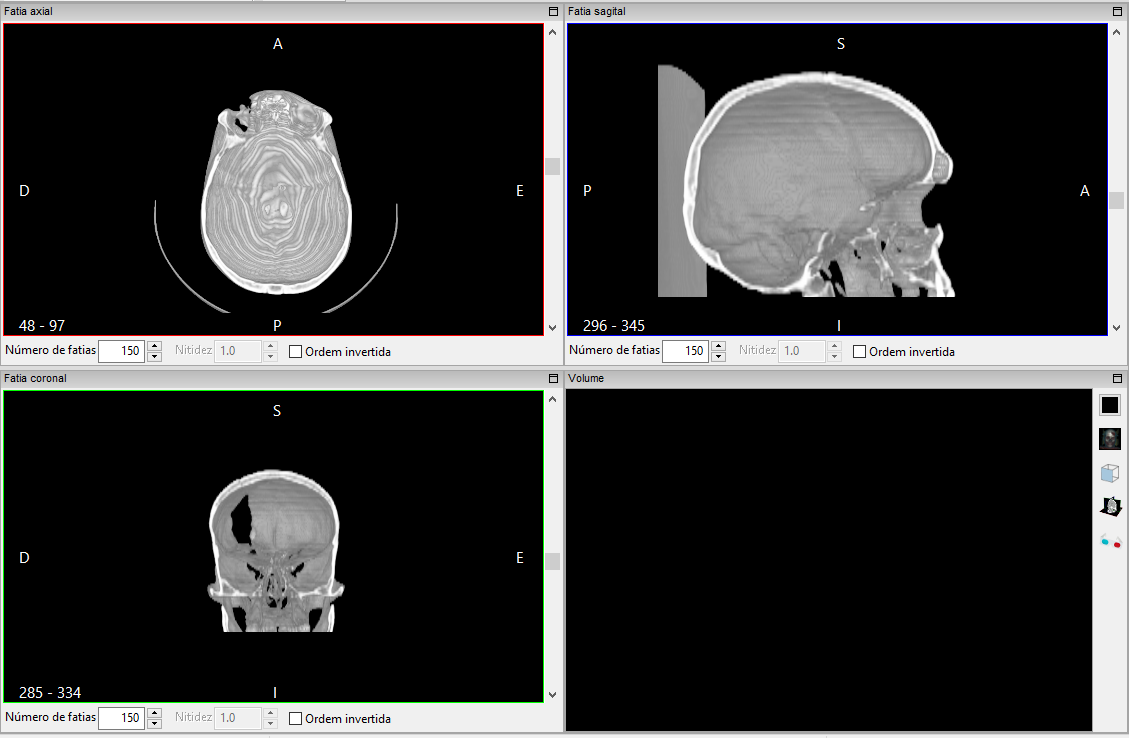
\includegraphics[scale=0.40]{multiplanar_window_mida_pt.png}
\caption{MIDA projection}
\label{fig:proj_MIDA}
\end{figure}

As the figure ~\ref{fig:proj_MIDA_inv} shows, it is possible to invert the order that the voxels are visited by selecting the option \textbf{Inverted order} in the lower corner of the screen.

\begin{figure}[H]
\centering
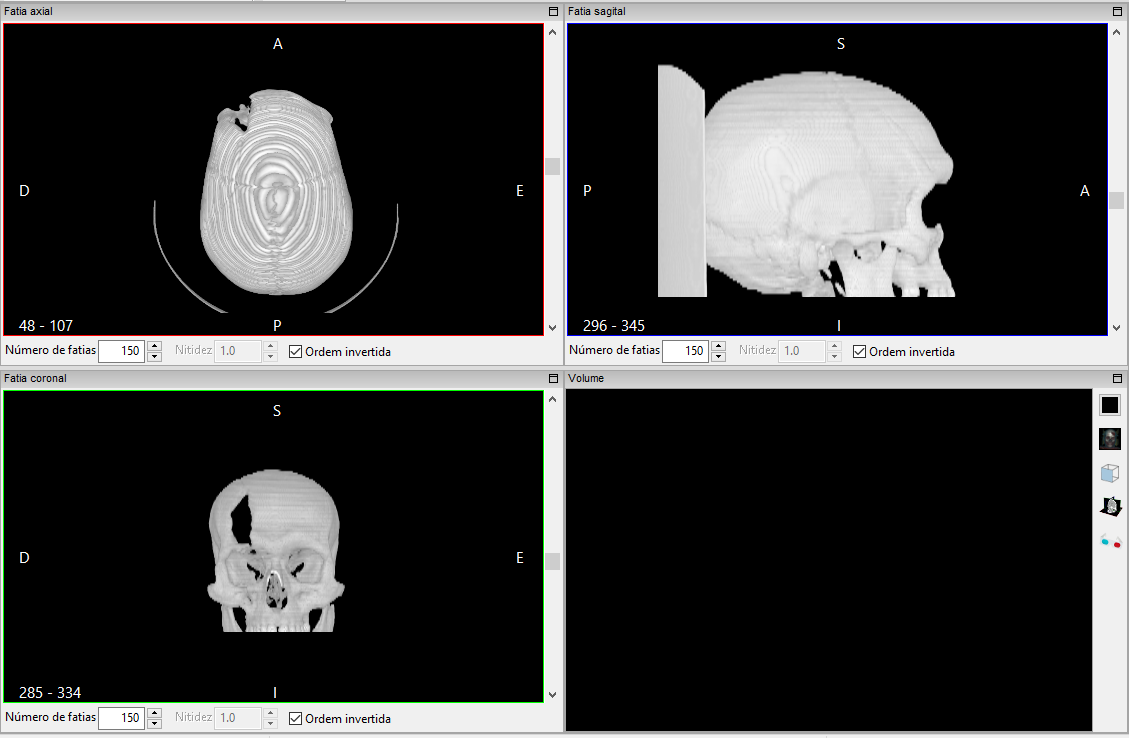
\includegraphics[scale=0.40]{multiplanar_window_mida_inverted_pt}
\caption{Inverted order MIDA projection}
\label{fig:proj_MIDA_inv}
\end{figure}

\subsection{Contour MaxIP}

The technique consists in visualizing contours present in the projection generated with MaxIP technique(\ref{sec:max_ip}). An example is presented in the figure~\ref{fig:proj_contorno_maxip}.

\begin{figure}[H]
\centering
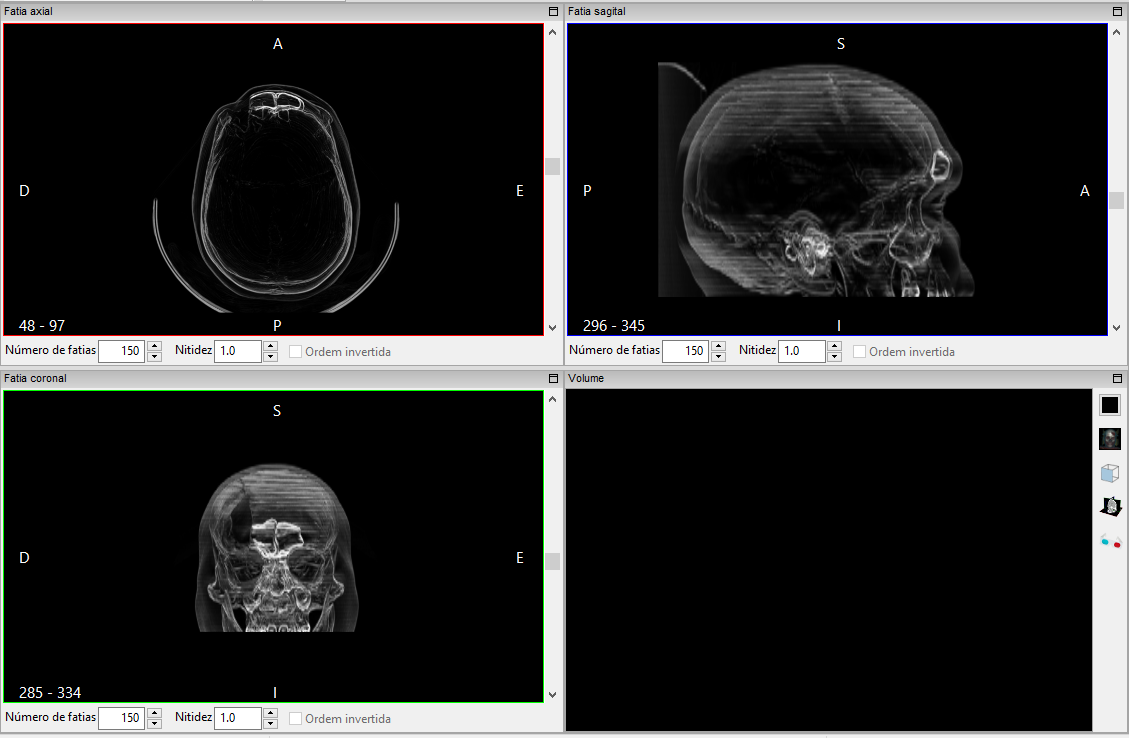
\includegraphics[scale=0.40]{multiplanar_window_contour_maxip_pt.png}
\caption{Contour MaxIP projection}
\label{fig:proj_contorno_maxip}
\end{figure}

\subsection{Contour MIDA}

The technique consists in visualizing contours present in the projection generated with the MIDA technique(\ref{sub:mida}). Like MIDA, you can reverse the order that the volume is visited. We exemplify in the figure~\ref{fig:proj_contorno_mida}.

\begin{figure}[H]
\centering
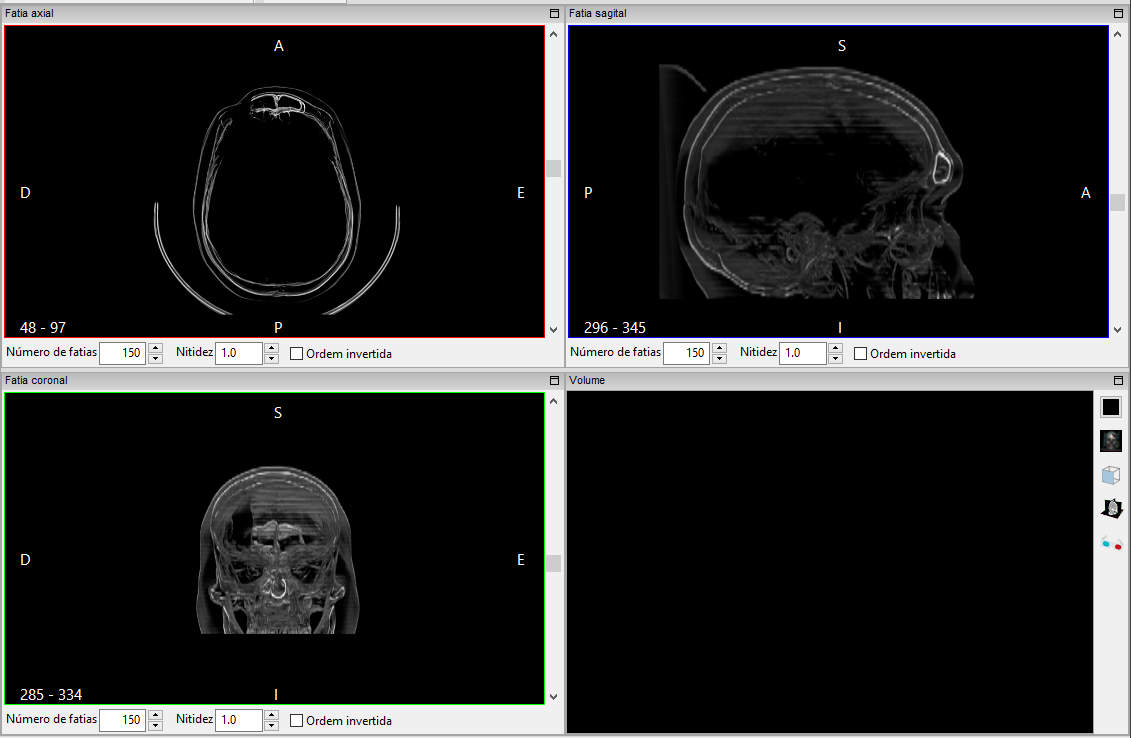
\includegraphics[scale=0.40]{multiplanar_window_contour_mida_pt.png}
\caption{Contour MIDA projection}
\label{fig:proj_contorno_mida}
\end{figure}